\begin{frame}{Ευθυγράμμιση πανοραμικών σαρώσεων από ευθυγράμμιση εικόνων;}

  {\small
  \texttt{FMI\_SPOMF} [1]: Fourier-Mellin Invariant (descriptor using) Symmetric Phase-Only Matched Filtering
  }

  \begin{figure}
    

\tikzset{every picture/.style={line width=0.75pt}} %set default line width to 0.75pt

\begin{tikzpicture}[x=0.75pt,y=0.75pt,yscale=-1,xscale=1]
%uncomment if require: \path (0,300); %set diagram left start at 0, and has height of 300

%Image [id:dp4534608740201713]
\draw (65.2,55) node  {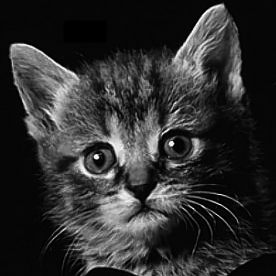
\includegraphics[width=52.5pt,height=52.5pt]{./figures/slides/ch5/cats/cat_1.png}};
%Image [id:dp1455593700628246]
\draw (65.6,136) node  {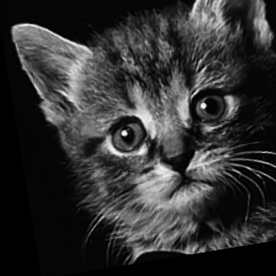
\includegraphics[width=52.5pt,height=52.5pt]{./figures/slides/ch5/cats/cat_2.png}};
%Image [id:dp2284961647386039]
\draw (286,95.5) node  {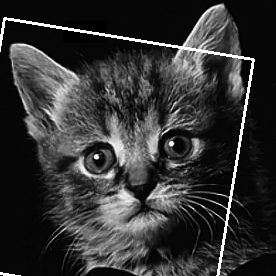
\includegraphics[width=52.5pt,height=52.5pt]{./figures/slides/ch5/cats/cat_3.png}};
%Straight Lines [id:da20924177841890534]
\draw    (100.25,56) -- (169.75,56) ;
%Straight Lines [id:da17546086467219557]
\draw    (100.25,136) -- (169.75,136) ;
%Straight Lines [id:da5388919164053374]
\draw    (169.75,55.5) -- (169.75,79.5) ;
\draw [shift={(169.75,81.5)}, rotate = 270] [color={rgb, 255:red, 0; green, 0; blue, 0 }  ][line width=0.75]    (10.93,-3.29) .. controls (6.95,-1.4) and (3.31,-0.3) .. (0,0) .. controls (3.31,0.3) and (6.95,1.4) .. (10.93,3.29)   ;
%Straight Lines [id:da31501738536372215]
\draw    (169.75,136.5) -- (169.75,113.38) ;
\draw [shift={(169.75,111.38)}, rotate = 90] [color={rgb, 255:red, 0; green, 0; blue, 0 }  ][line width=0.75]    (10.93,-3.29) .. controls (6.95,-1.4) and (3.31,-0.3) .. (0,0) .. controls (3.31,0.3) and (6.95,1.4) .. (10.93,3.29)   ;
%Straight Lines [id:da39659823711660636]
\draw    (221.89,95.88) -- (246,95.88) ;
\draw [shift={(246,95.88)}, rotate = 180] [color={rgb, 255:red, 0; green, 0; blue, 0 }  ][line width=0.75]    (10.93,-3.29) .. controls (6.95,-1.4) and (3.31,-0.3) .. (0,0) .. controls (3.31,0.3) and (6.95,1.4) .. (10.93,3.29)   ;
%Straight Lines [id:da03488873963603334]
\draw    (221.39,100.25) -- (233,100.25) ;
%Straight Lines [id:da8480911956167825]
\draw    (233,99.75) -- (233,155.38) ;
\draw [shift={(233,157.38)}, rotate = 270] [color={rgb, 255:red, 0; green, 0; blue, 0 }  ][line width=0.75]    (10.93,-3.29) .. controls (6.95,-1.4) and (3.31,-0.3) .. (0,0) .. controls (3.31,0.3) and (6.95,1.4) .. (10.93,3.29)   ;

% Text Node
\draw    (130.66,84) -- (221.66,84) -- (221.66,109) -- (130.66,109) -- cycle  ;
\draw (176.16,96.5) node   [align=left] {\texttt{FMI\_SPOMF}};
% Text Node
\draw (173,164) node [anchor=north west][inner sep=0.75pt]   [align=left] {$(\Delta x, \Delta y)$, $\Delta \theta$, $\sigma$, $w$};

\draw (65.2,10) node {Αρχική, $\texttt{I}_1$};
\draw (65.2,181) node {Μετασχηματισμένη, $\texttt{I}_2$};
%\draw (265.2,6.5) node {\tiny $Q(\theta, \lambda) = \dfrac{\mathcal{F}\{\texttt{I}_1\}^{\ast} \odot \mathcal{F}\{\texttt{I}_2\}}{|\mathcal{F}\{\texttt{I}_1\}| \cdot |\mathcal{F}\{\texttt{I}_2\}|} = e^{-i (\phi_2-\phi_1)} = \exp^{-i \cdot \Delta\theta}$} {};

%\draw (255.2,6.5) node {\tiny $Q(\theta, \lambda) = \dfrac{\mathcal{F}\{\texttt{I}_1\}^{\ast} \odot \mathcal{F}\{\texttt{I}_2\}}{|\mathcal{F}\{\texttt{I}_1\}| \cdot |\mathcal{F}\{\texttt{I}_2\}|}$} {};
%\draw (255.2,30) node {\tiny $\Delta \theta = \operatorname*{arg\,max}\limits_\theta \mathcal{F}^{-1}\{Q\}$} {};
%\draw (255.2,40) node {\tiny $\sigma = \exp{\operatorname*{arg\,max}\limits_\lambda \mathcal{F}^{-1}\{Q\}}$} {};
%\draw (255.2,50) node {\tiny $w = \max \mathcal{F}^{-1}\{Q\}$} {};


\end{tikzpicture}


  \end{figure}


\begin{textblock}{14}(12.6,6.5)
{\tiny $Q(u,v) = \dfrac{\mathcal{F}\{\texttt{I}_1\}^{\star} \cdot^\ast \mathcal{F}\{\texttt{I}_2\}}{|\mathcal{F}\{\texttt{I}_1\}| \cdot |\mathcal{F}\{\texttt{I}_2\}|}$}\\
{\tiny $q(\theta, \lambda) = \mathcal{F}^{-1}\{Q\}$}\\
{\tiny $\Delta \theta = \operatorname*{arg\,max}\limits_\theta q$}\\
{\tiny $\sigma = \exp{\operatorname*{arg\,max}\limits_\lambda q}$}\\
{\tiny $w = \max q$}
\end{textblock}

  \placebottom
  \tiny
  [1] Qin-Sheng Chen, M. Defrise and F. Deconinck, ``Symmetric phase-only matched filtering of Fourier-Mellin transforms for image registration and recognition," \textit{IEEE Transactions on Pattern Analysis and Machine Intelligence}, 1994



\note{\footnotesize
Μέσα από την αναζήτησή μας βρήκαμε τη μέθοδο FMI-SPOMF, η οποία χρησιμοποιείται
στον κλάδο της υπολογιστικής όρασης για την εκτίμηση ανάμεσα σε δύο εικόνες
της μετατόπισης τους, της γωνίας περιστροφής τους, της κλιμάκωσης
τους, και του βαθμού ομοιότητάς τους. Αυτές οι παράμετροι υπολογίζονται με
κλειστό τρόπο και χωρίς να υπολογίζονται αντιστοιχίσεις ανάμεσα
στις δύο εικόνες.}

\end{frame}
